\chapter{Discussion}\label{chap:discussion}

In this chapter, we will report what we have managed to do this semester as part of the project and preparation for next semester's master's thesis. We will firstly report our results from the data collection and systematic literature reviews whose methods were described in chapter \ref{chap:method}. Then, we will go through the identified challenges and precautions we must take in regards to the system we will develop. Lastly, we briefly mention our work in the theory modules before describing our current plan and vision for a prototype of our system.

\begin{comment}
The results chapter should simply present the results of applying the methods presented in the method chapter without further ado. This chapter will typically contain many graphs, tables, etc. Sometimes it is natural to discuss the results as they are presented, combining them into a `Results and Discussion' chapter, but more often they are kept separate.

Here you should discuss all aspect of your thesis and project. How did the process work? Which choices did you make, and what did you learn from it? What were the pros and cons? What would you have done differently if you were to undertake the same project over again, both in terms of process and product? What are the societal consequences of your work?

IT2810 - Web development
IT3021 - Game+
TET4205 - Power system analysis 2
IT3402 - Service design
Trond Morten

Innsida - Two reached out, one provided data
Excited - No response
Contact persons - 3
Co-supervisor contact - 1
Backup - Peer reviews

Do we have enough data?
\end{comment}

\section{Collected data}
% Write about what we know about the data. In the final thesis, have a more in-depth analysis

As described in section \ref{sec:data-collection-strategy}, we have reached out to potential collaborators through a few different fora with the goal of collected open-text responses submitted by students through response systems.

Firstly, our attempt at reaching out to the members of Excited did not yield any result. As for the note published on Innsida, we had two lecturers reach out to us. One of them, a lecturer of an electrical engineering course, has collected open-text responses through Mentimeter this semester at regular intervals and shared the responses with us. The obtained dataset contains various types of questions, such as multiple-choice and scales, but also open-text questions. There are in total 337 responses written in English. The length varies from a single word to a couple of short sentences.

In terms of lecturers we have reached out to directly, we have received responses from three, all within the domain of computer science. Two of the datasets are quite small. The first of them consists of 24 Norwegian responses distributed over three questions. The second consists of eight responses in Norwegian also distributed over three questions. Both datasets are collected through Mentimeter. These two datasets are hardly large enough to be of much use, as it is easy for a lecturer to look through all the responses to a question during a lecture; there is no need for any computer-assisted analysis of the responses. The third dataset, on the other hand, is more extensive. It contains 15 questions with 478 English responses with between 19 and 43 responses per question. The responses vary from a single word to a short sentence. An interesting feature of this dataset is that some responses contain emojis, which is something that our system must handle.

The last collected dataset was shared with us by a contact of our co-supervisor. They are also a lecturer at NTNU, and the dataset contains around 1000 responses collected over a few years in engineering courses. The responses are mainly in Norwegian. We are currently not in possession of this dataset, but we will receive it before starting experimentations next semester.

In conclusion, we have managed to collect three datasets of sufficient size - around 1800 responses - and a sufficient number of responses per question for them to be valuable during experimentation with text mining methods. We also have both English and Norwegian responses. At this point in time, we have not yet analysed the datasets. In the final master's thesis, we will include a thorough analysis of the collected datasets.

\section{Systematic literature review}\label{sec:results-slr}
% Talk about the plans for the SLR for the next semester
% Mention resources, search string, number of results, exclusions
In this section, we will present the results we have thus far from our SLR. We will also explain what is missing at this point in time and lay out the road ahead for the upcoming semester, spring 2025.

\subsection{Study selection}
% Describe the results of the search and selection process, from the number of records identified in the search to the number of studies included in the review, ideally using a flow diagram
Following the selection process outlined in section \ref{sec:slr-selection-process}, we obtained the results as shown in the PRISMA flowchart of figure \ref{fig:prisma-flowchart}.

\begin{figure}[h!]
    \centering
    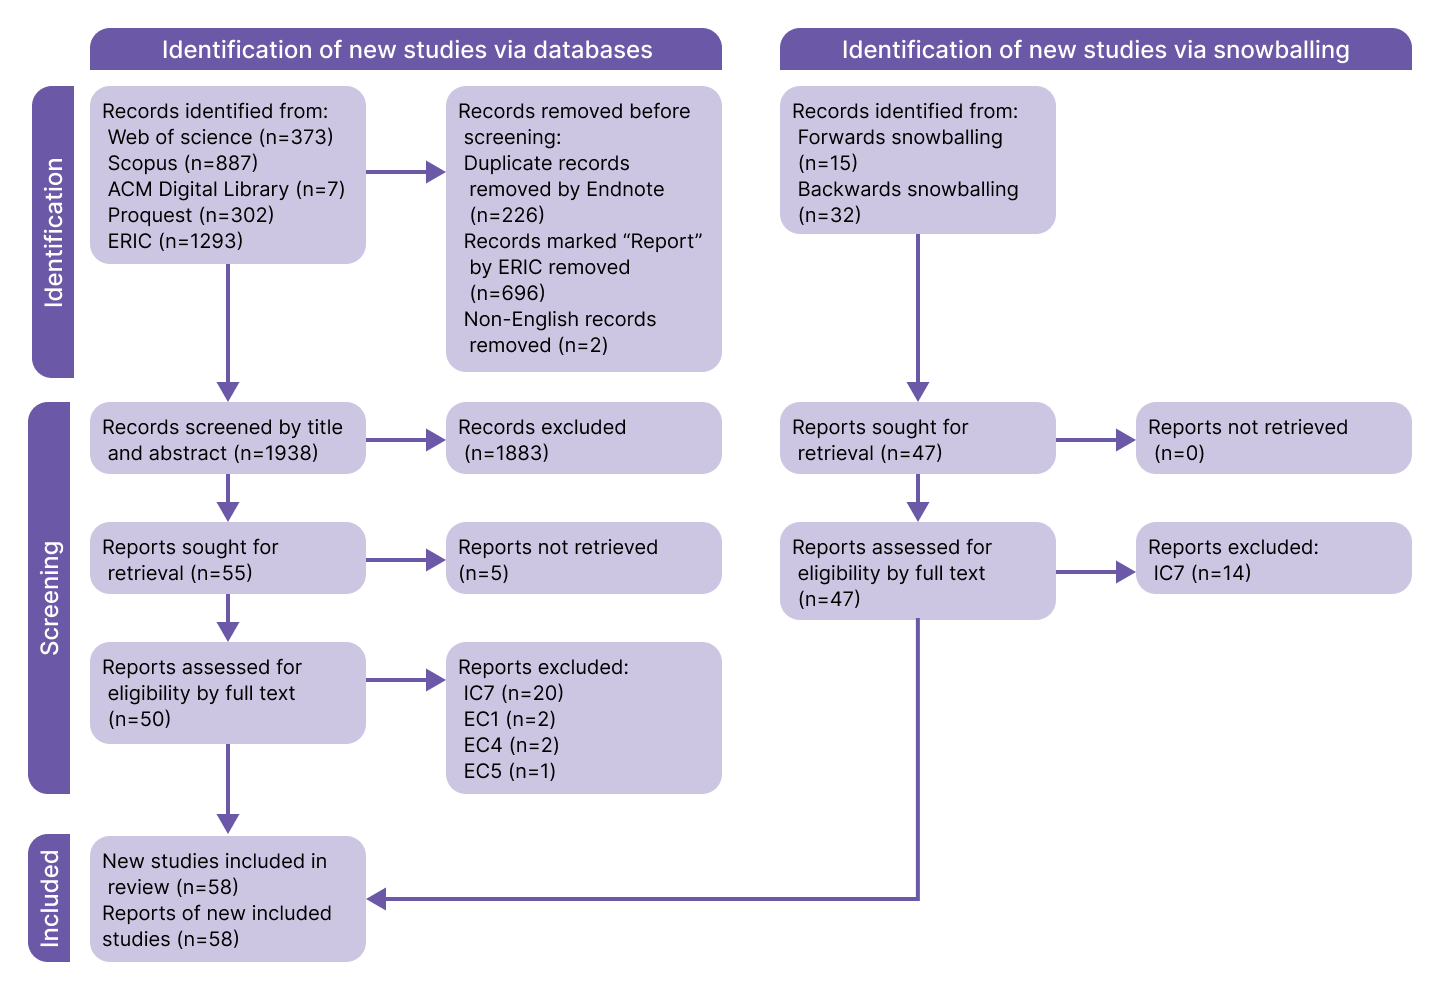
\includegraphics[width=\textwidth]{figures/PRISMA diagram.png}
    \caption{PRISMA flowchart depicting the results of the study selection process.}
    \label{fig:prisma-flowchart}
\end{figure}

When we entered our search query into the five scientific literature databases and applied the respective filters and limits, we ended up with a total of 2862 papers. 373 of these came from Web of science, 887 from Scopus, only seven from ACM Digital library, 302 from Proquest and 1293 from ERIC. After having exported all the papers to Endnote, we noticed that 696 of the papers coming from ERIC were marked as reports instead of journal articles, despite having set the \textit{Journal articles} filter. These were removed, as we are interested in papers describing new research. After that we used Endnote's built-in functionality to remove duplicates, which resulted in 226 fewer papers. Lastly, two papers were removed that were not in English, leaving us with 1938 papers for screening.

When screening the titles and abstracts, we applied the eligibility criteria. 1883 papers were excluded after this, leaving 55 papers. Five of these did not have full text available. 50 papers were subsequently full text screened and the exclusion reason reported. For the IDs of the eligibility criteria refer to table \ref{tab:eligibilitycriteria}.

We, thereafter, performed an iteration of forwards and backwards snowballing on the 25 papers that were included after full text screening. 15 papers were found through forwards snowballing, which is to say through the papers' citations, and 32 through backwards snowballing, which is to say through the papers' references. Some papers appeared both in citations and references, in which case they are reported as coming from backwards snowballing. Papers that were already found through searching the databases were immediately excluded as duplicates and not part of the reported statistics in figure \ref{fig:prisma-flowchart}. Snowballing resulted in 47 new papers, of which 14 were excluded due to them not fulfilling inclusion criterion IC7. We were then left with 33 papers from snowballing, with the total count of included papers being 58. These 58 went on to be part of the data extraction process.

While these 58 papers are all published in the period 2015-2024, we have compiled the bar chart in figure \ref{fig:papersbyyear} to get an idea of the papers' timeline. Most of the papers were published in 2019, 2023 and 2020. However, the chart shows no significant trend.

\begin{figure}[h!]
    \centering
    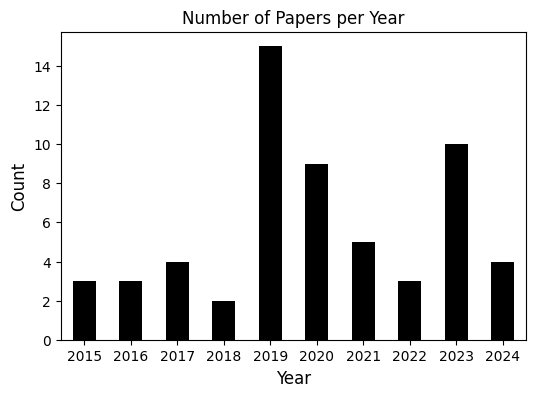
\includegraphics[width=.8\linewidth]{figures/papers-by-year.png}
    \caption{Distribution of included papers by publication year}
    \label{fig:papersbyyear}
\end{figure}

\subsection{Data extraction}
Despite the data extraction not being fully completed, we can comment on what we have extracted so far. Of the 58 included papers, ten have still not had data extracted. We have not yet performed any analysis on the data. The reporting in our Excel document regarding the codes, does not yet lend itself to easy data analysis due to formatting, misalignments in the use of codes and their naming, and some blank rows and cells. We find that it is better to perform a proper analysis when the data extraction process is at a more mature stage.

A first observation we have made is the lack of studies using response systems for data collection. This is in line with the impression we had in the early phases when searching scientific databases in a less structured way for literature and as we have commented upon in chapter \ref{chap:relatedwork}. From the 48 papers with data extracted, only a single paper has been coded with ``Response system'', and this study only uses response systems as one of two systems for collecting open-text responses, the other being feedback comments from the MOOC Coursera. On the other hand, there are 15 papers marked as having a ``Synchronous'' learning environment, i.e. that the data is collected in a live classroom or lecture setting. In all cases, the open-text analysis is performed with text mining tools by the researchers at a later point, but the data in these 15 studies can still be considered more representative of a real-time response system scenario than data collected from surveys, MOOC comments or reviews asynchronously. Though the data collection is synchronous, what system is used differs. Five papers simply mention that the data was collected during class or a lecture without saying how. Three used online surveys, such as Google form, two used a learning management system in some way, and four used some form of mobile app, and one used a response system. One can argue that the learning management systems and mobile apps act as response systems, in which case we have seven studies investigating open-text responses collected through response systems. This is why we need to further refine and discuss the codes used, to simplify the data analysis and agree on what is considered a response system and not.

A second observation we can make is which AI methods are used. So far we have identified four AI tasks and a good amount of AI algorithms corresponding to these tasks. Keep in mind that the number of papers with each code is subject to change as we progress in the data extraction process.

\begin{itemize}
    \item \textbf{Topic modelling:}
    19 of the papers have been coded with ``Topic modelling''. Topic modelling is the act of grouping text documents - such as open-text responses or single sentences - into a given number of themes based on semantic similarity. We have decided to include both unsupervised, semi-supervised and supervised AI methods in our definition. Some of the algorithms identified for the use of topic modelling are Latent Dirichlet Allocation (LDA), K-means and K-Medoids. LDA has been used by several studies both in its unsupervised form and in a semi-supervised form where seed words are used to guide the discovery of themes.
    \item \textbf{Sentiment analysis:}
    27 papers are coded ``Sentiment analysis'', which appears to be the most used approach to analysing open-text responses in education. Sentiment analysis includes any AI method for extracting feelings, emotions or sentiment scores from text. Both lexicon-based and machine learning-based algorithms have been used. Lexicon-based sentiment analysis calculates scores for how negative, neutral or positive some piece of text is using a lexicon of words annotated with per-word sentiment scores. Some lexicons that are used are the MPQA corpus, SentiStrengthId, NRC emotion lexicon, Afinn lexicon and the VADER lexicon. VADER has been the most prominent one among the included papers. For machine learning, some used methods are Decision trees, Naive Bayes, Support Vector Machine, K-Nearest Neighbour, Random Forest, and various BERT-based models. Many of these are more general text classification models, but since sentiment analysis is employed to such a great extent, we have decided to set it as its own AI task instead of referring to it as simply text classification.
    \item \textbf{Text classification:}
    10 papers have the code ``Text classification''. Text classification is the act of assigning pieces of text to pre-defined classes or categories. Classification of sentiments is considered as sentiment analysis instead of text classification. Some employed AI methods in this regard are different rule-based classifiers, conditional inference trees, logistic regressions, Markov Random Field, as well as some of the ones used for sentiment analysis.
    \item \textbf{Text summarisation:}
    4 papers deal with ``summarisation''. Summarisation is a broader task than the three others and may use classification, topic modelling or sentiment analysis as part of the process. The task concerns itself with providing a textual summary over all input text. This can either be abstract, where new text is generated, or extractive, where pieces of the input text are extracted and put together into a summary. These papers use an array of the aforementioned AI methods in addition to methods such as LexRank for ranking pieces of text according to relevance.
\end{itemize}

Another relevant observation is the proposed future work reported by the included papers. What appears to be the the most commonly mentioned one, is to increase generalisability. This means that the AI methods in the study should be tested on more diverse data, for instance, on different courses, with different natural languages or a larger sample size. Somewhat related to this, a few studies reported that the evaluation process needs to be improved to be more certain of how well the AI methods perform. Another rather common mention was to increase granularity. Several studies found that performing, for instance, sentiment analysis over all open-text responses did not give enough insight. As such, performing sentiment analysis over each topic could give more insight into why the students feel a certain way. To help with insight, some studies also saw the need for developing or improving visualisations, usually in the form of dashboards. Yet another future work that was mentioned by several papers was to analyse non-textual data together with the textual data. This could be in the form of numerical data, such as exam grades or likert-scale responses, or it could be video or audio recordings. We can also add improving performance of the methods and extending the current system with more features. Exactly what is referred to here depends very much on the text mining method or system developed and tested in the study. Examples can be to create a more domain specific sentiment lexicon, combine individual methods into a a bigger system, extend with multilingual support and reduce dimensionality and resource requirements.

\subsection{Current status}
As mentioned, the work on the SLR is not completed and will resume in the spring semester 2025, with the aim of publishing it eventually on the side of the master's thesis. At this point in time, we have completed the study selection, and we have carried out data extraction for most of the 58 included papers. The data extraction still requires some work, however. We will in the following attempt to explain the next steps for the SLR.

\begin{enumerate}
    \item \textit{Quality assessment}: The quality of the included papers must be assessed. For this we must develop some quality assessment rules to be applied on all 58 papers. This will ensure that the papers contain sufficient information for our needs and that the results of the studies are truly relevant for our SLR.
    \item \textit{Research questions}: While we have an outline for what data shall be reported in the SLR and an idea of what the SLR should accomplish, we still need to define concrete research questions that can be answered during synthesis of the results.
    \item \textit{Finish data extraction}: We have already extracted data from 48 or the 
    58 included papers, but the codes need to be refined further to make the reporting of the data more meaningful and valuable. The remaining papers need to have data extracted and the formatting of the Excel document must be formatted to make data analysis easier.
    \item \textit{Data synthesis}: After reporting the extracted data, we must make sense of the findings and use the insight to answer our research questions.
    \item \textit{Write the paper}: When we have answered our research questions, the paper itself must be written. This will include explaining the rationale of our SLR, present our research questions and why they are relevant, present the employed SLR methodology, report the results of the paper selection process, report the data from the included papers, answer the research questions, and conclude on what we have achieved with the SLR.
\end{enumerate}

Until now, we have been three people working on this SLR. This includes the two of us - in the form of two master students - and a PhD candidate. In the coming semester, the work will mainly be conducted by the PhD candidate while we focus on the master's thesis. To perform our experiments on the collected open-text data next semester, we will be dependent on using insights from the SLR as a guide in choosing which AI methods to test, which pre-processing steps and tools may be effective and how different AI methods can be combined to provide more actionable insights from the open-text data.

\section{Proprietary solutions}
In addition to consulting literature, we have looked into how the two response systems, Mentimeter and Kahoot!, use AI to analyse open-text responses.

Mentimeter provides two options for analysing open-text responses using AI. The summary feature can be used for the open-ended and word-cloud question types. After a few seconds of processing, Mentimeter will provide a summary in the form of a handful of key points, each around five words with a suitable emoji. The summary feature is briefly explained in \cite{mentisummary}. The grouping feature, explained in \cite{mentigrouping}, can be used for the open-ended question type. If a question has more than ten responses, they can be grouped according to themes. Labels are automatically assigned to each group, and the user can select a group to see the related responses. Except for explaining these features themselves, Mentimeter does not provide any information on how they are implemented, however, from what we have found.

Kahoot! uses AI for clustering ideas submitted in response to their brainstorming question type. One of the developers at Kahoot!, who took part in implementing the clustering algorithm, explains how it works in \cite{kahootclustering}. He explains here that they have chosen an unsupervised clustering method. It uses the \textit{xlm-r-bert-base-nli-stsb-mean-tokens} model from the \textit{Sentence Transformers} Python library to create embeddings for the open-text responses. These embeddings are vector representations optimised for comparing semantic similarity between pieces of text. They then use a classical clustering method - he mentions \textit{K-means} in the article - and follow the \textit{elbow method} with a few optimisations to choose the appropriate number of clusters. As they had performance problems due to high dimensionality, they applied the \textit{TruncatedSVD} module from the \textit{scikit-learn} library to reduce it. While this algorithm has worked well, the article, which is from 2022, underlines that updates are in order. Newer transformer models have been made available and should be tested, auto-encoders should be explored to help reduce dimensionality of the embeddings, and other clustering algorithms should be checked out, such as \textit{HDBSCAN} and \textit{FAISS}.

All of these features are tried and tested in practice, which goes to show that real-time analysis of open-text responses through response systems is, indeed, viable. While Mentimeter and Kahoot! have implemented clustering and summarisation, we intend to look into more methods, such as sentiment analysis, as well as whether methods can be combined.

\section{Implementation challenges and precautions}
From the literature and from other observations we have made during the work on the project, we have identified a handful of factors that we must take into account when developing the our system. The lack of literature on applying text mining methods to open-text responses from a response system, means that we have few examples to draw inspiration from directly. The most tried and true example seems to be the clustering algorithm developed by Kahoot!. While we can and will draw inspiration from the other collected literature, almost none of the papers have been faced with the real-time aspect of text mining, nor the use of it in a live physical classroom or lecture hall. We must, therefore, be careful to manage the dimensionality of our AI models and ensure that they are able to process the responses within, preferably, less than a minute. This will also make it difficult to train machine-learning models due to lack of relevant data and the instructor should not need to perform any manual analysis, such as labelling the clusters. Furthermore, we need to figure out what visualisations would be useful for an instructor and the students for them to gain useful and actionable insights into the open-text responses while in an ongoing class or lecture. This will contribute to decide which text mining methods to use and what post-processing to perform.

While far from exclusive to our case, we must deal with various potentially problematic characteristics of the open-text responses that the system will receive. We must here consider typos, diacritics, emojis, emoticons, profanities, unserious and off-topic responses, ``shouting'', mixing of languages, typing in none-standardised dialect and more. It will be necessary to handle multiple languages, as well. In our case, this will be English and Norwegian. Compared to languages like English, Chinese, Arabic, Spanish and German, Norwegian is a rather small language that may not have as many resources for use in text mining. We are here talking about, for instance, lexicons and corpora for sentiment analysis, support in text mining libraries for pre-processing, filter lists, and pre-trained machine learning models.

\section{Work from theory modules (TDT06 \& TDT07)}
In the theory modules we explored and investigated the domain of educational data analysis and dashboard design, with the goal of enhancing student engagement and performance. The primary focus was related to a dataset that monitored the usage of an educational dashboard in the context of performing a course related quiz. Our data analysis revealed that increased usage of dashboard was correlated to better academic scores. The dataset also contained information on question difficulty, and we could determine that all kinds of questions benefited, even though the most difficult questions had slightly more improvement.

Building on these findings, we developed a prototype of a new educational dashboard solution in Figma, as can be seen in \ref{fig:previous-work-theory-modules-prototype}. Since dashboard usage was a major factor in educational performance, we designed the prototype with a goal of making the user want to use the dashboard more. We made sure that metrics, like progress-tracking, quiz accuracy and time-management, were clearly visible, so that the user could become aware of, and also see progress. Our hypothesis was that being able to see your own progress would make it more motivating to use the dashboard, and thus again increasing student performance. The dashboard also incorporated features to make performance feedback more actionable, aligning with principles of gamification and metacognitive feedback.

\begin{figure}[h!]
    \centering
    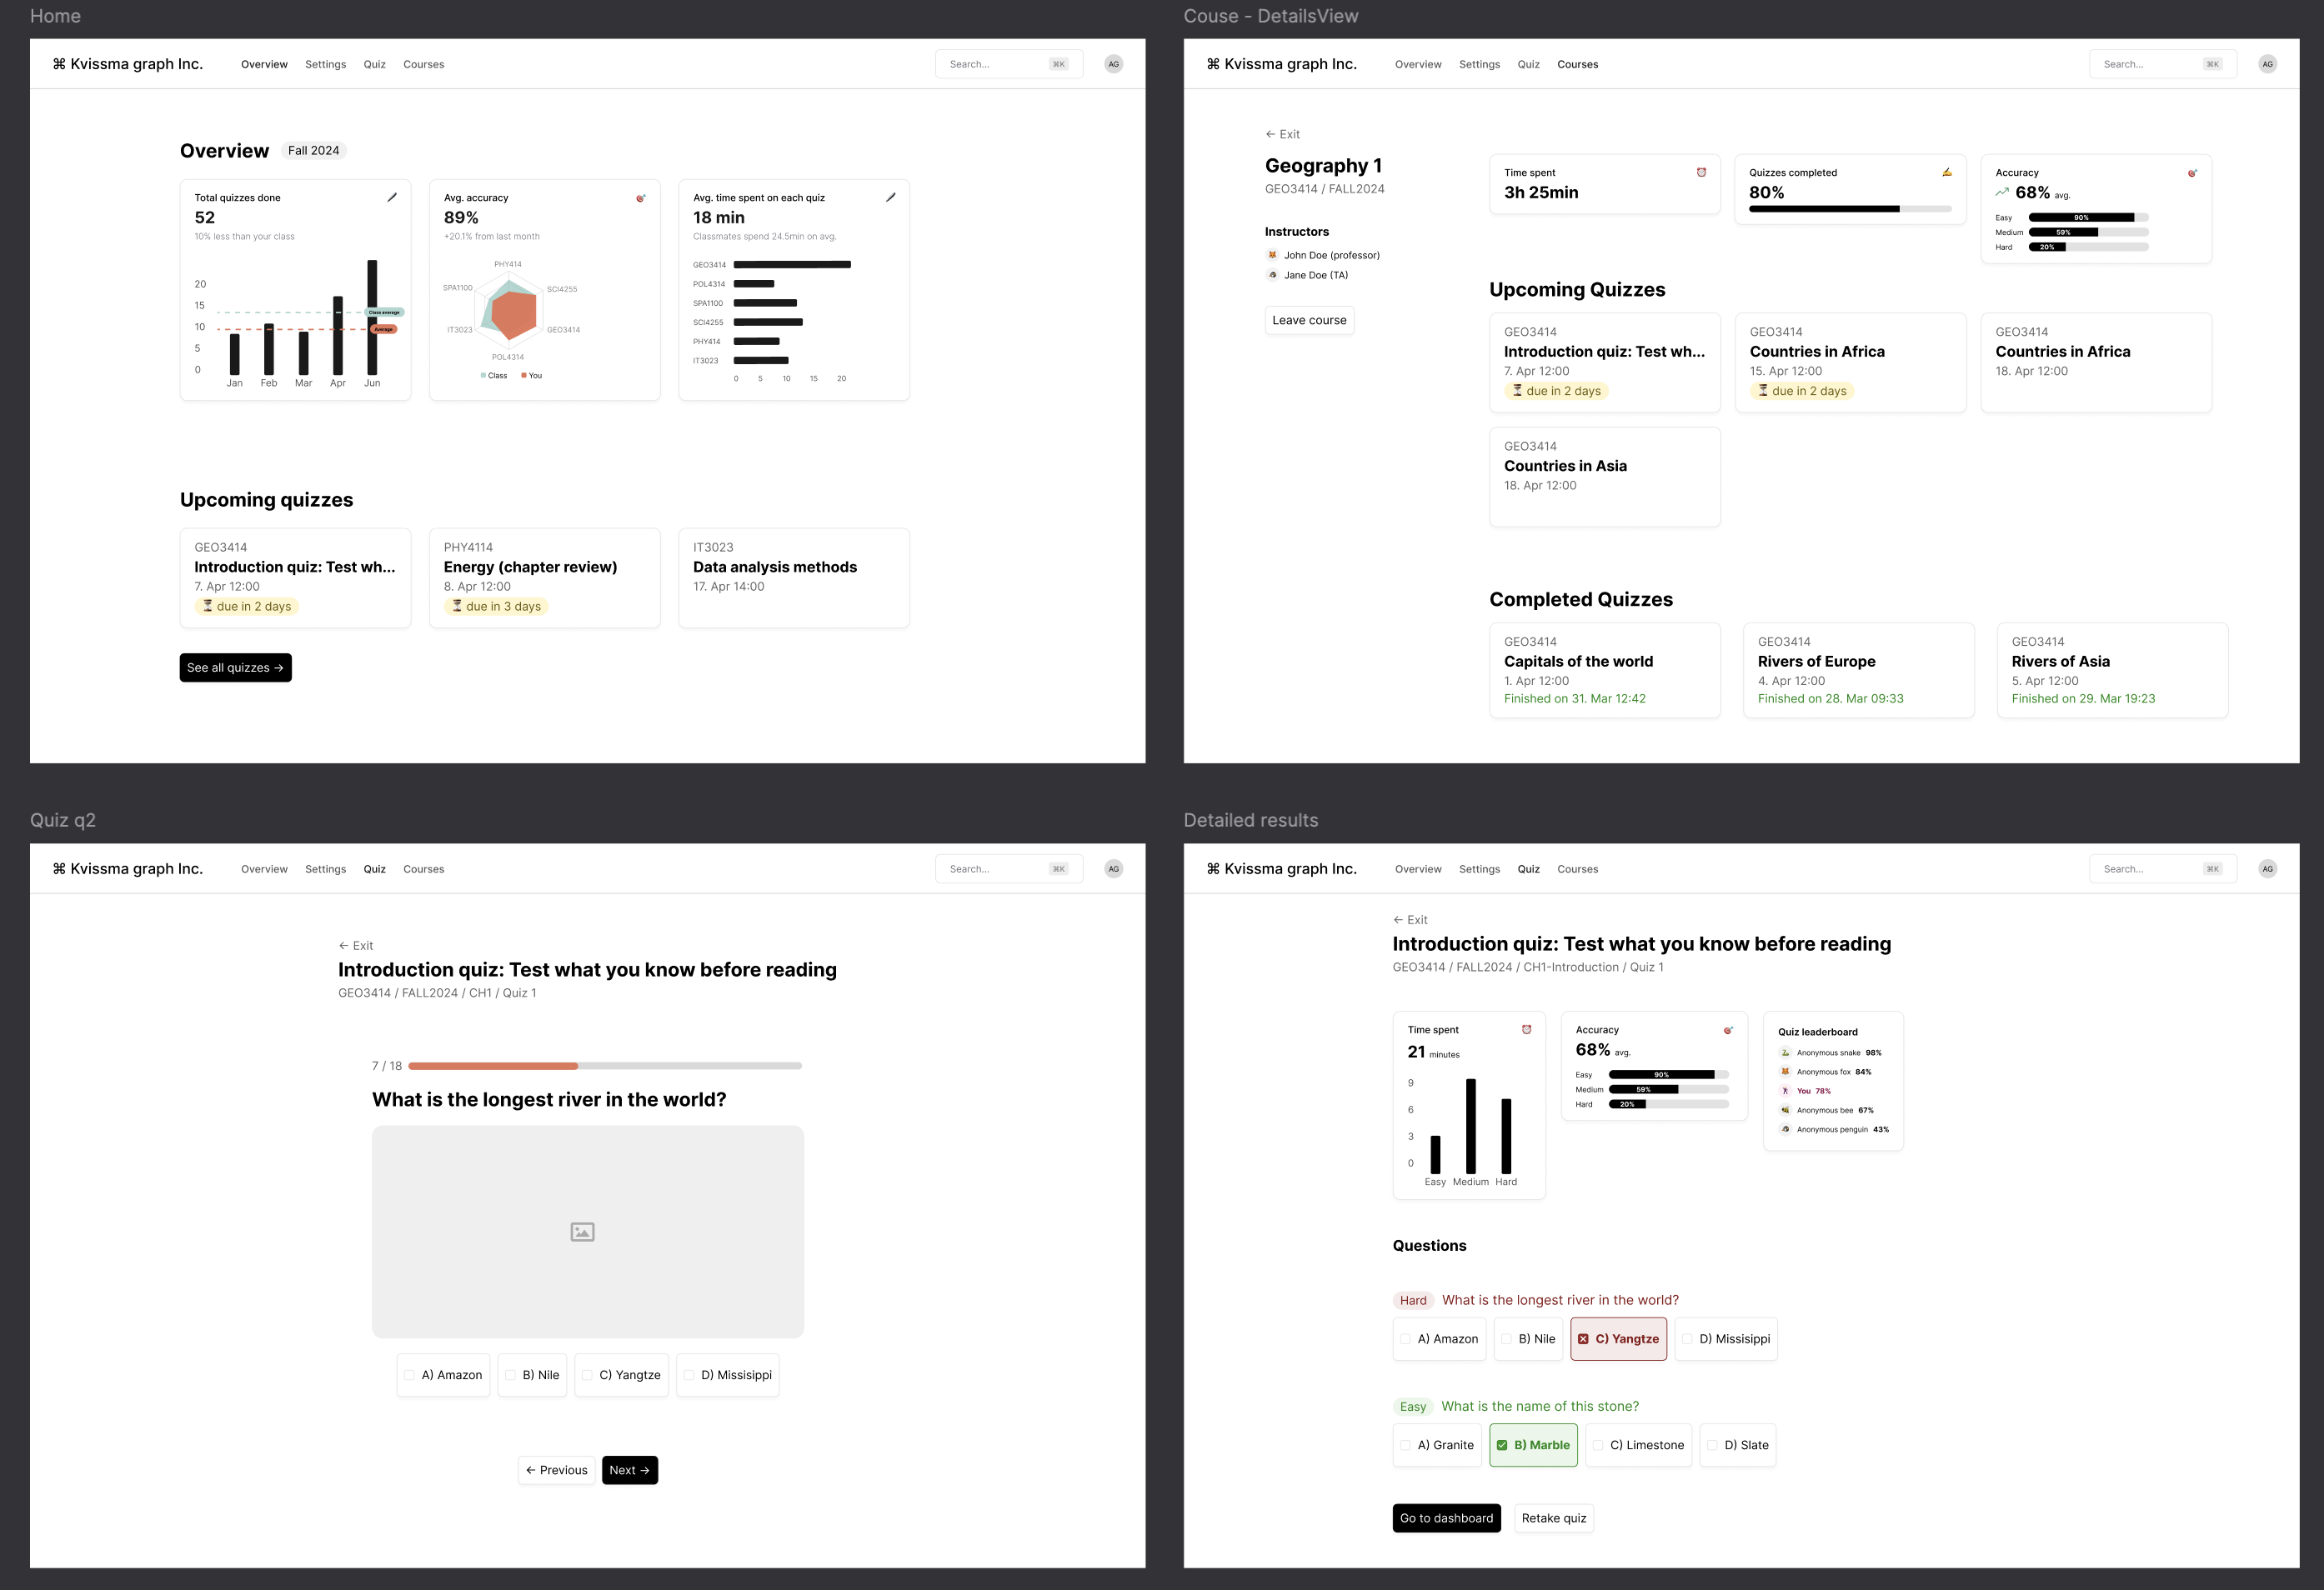
\includegraphics[width=1\linewidth]{figures//c5/previous-work.png}
    \caption{Some of the screens in the prototype we built in the theory modules \cite{theoryModule3}}
    \label{fig:previous-work-theory-modules-prototype}
\end{figure}

\section{Work from a previous master's thesis}
We have been informed by our supervisors regarding a previous master's thesis \cite{Olsen2024}. The thesis implemented a high-performant and scalable system designed to collect and display digital submissions from students in the same kind of environment as we focus on. The thesis consists of a software project with a backend and multiple frontends and services that together works like a streamlined classroom interaction tool that can handle textual submissions from students in a scalable and efficient way.

The ideal scenario would be that our project is built directly into this scalable system. However, due to our needs of rapid development and prototyping, we have found it more beneficial to create our own simple services from scratch, which then later can be migrated or incorporated into the architecture. We have not been able to contact the writer of the thesis regarding use of and best practices related to the system, further strengthening our decision of building our own system from the ground up. We believe that it is more important that we get a working prototype that can be tested in real classrooms, rather than having an optimised, performant solution. We will still make sure that our services will be able to handle enough load to support at least a single classroom session at a time.

\section{Plans for prototype}
We plan to create a functional proof-of-concept based on our prototype. Feature-wise it will consist of being able to create question-sessions, a classroom view where the teacher can ask questions, as well as a participant client that allows for joining a session and answering questions. With functionality consisting of sessions, collecting responses, and processing and displaying the result. To increase engagement we will add screens that incorporate visualisations of statistics and statements.  

The processing of the student responses will consist of a custom implementation of text-mining methods. We do not plan to design new algorithms for these features, but rather implement and combine them in a context where they are most effective in a classroom setting. 

We will split our prototype up in three pieces, host-frontend, client-frontend, backend. This autumn, we have created a Figma prototype of the frontend and a plan for features of the backend. We plan to develop both frontends in React, as it is the most widespread frontend framework and is sufficient for the needs of our technical requirements. It is also the frontend framework with which we are the most familiar. Since the choice of framework will not impact the prototype in any specific way, we chose the one best suited to our skill set so that we can spend the least amount of time on technical frontend development.

We will also strive in making sure both frontends are designed user-centric, responsive and accessible. We plan to do iterations based on user-feedback. The extent of this process will be determined based on the initial user-feedback. We will design a mobile-first approach since the majority of users will use a phone. We plan to do simple user testing with corresponding interviews. We plan to use a frontend library with support for custom styling and accessibility features out of the box, like, for instance, Radix Primitives or React Aria.

\subsection{Host frontend}
We will create a host frontend that allows the user to create, host and view previous sessions. This frontend will be used by the instructor. The frontend will support user-registration and authentication. For our prototype, only a simple form of username and password combination will be incorporated.

After authenticating and logging in, the user will be able to start new sessions. When the session opens, it will display a six letter session-code that users can enter to join the session. This screen is intended to be shared with the audience to ensure a smooth user experience. This can be done either via a TV screen or by broadcasting it to a digital platform. Then, the organiser can ask the audience questions in a format that looks familiar to sending a text message, while still sharing the same screen. In the first stage, we will only allow the host to create questions live. In a more polished system, the host would also be able to set up the questions ahead of the lecture.

The submissions from the audience will be displayed on the screen instantaneously, and after enough responses have been received, the system will begin to analyse results. For instance, the system will try to group similar inputs together, as well as utilising a mix of text mining methods - determining exactly which methods to use will be an important part of the work on the master's thesis the coming semester. The result of this processing will be visible after the countdown is finished.

\clearpage
\begin{figure}[h!]
    \centering
    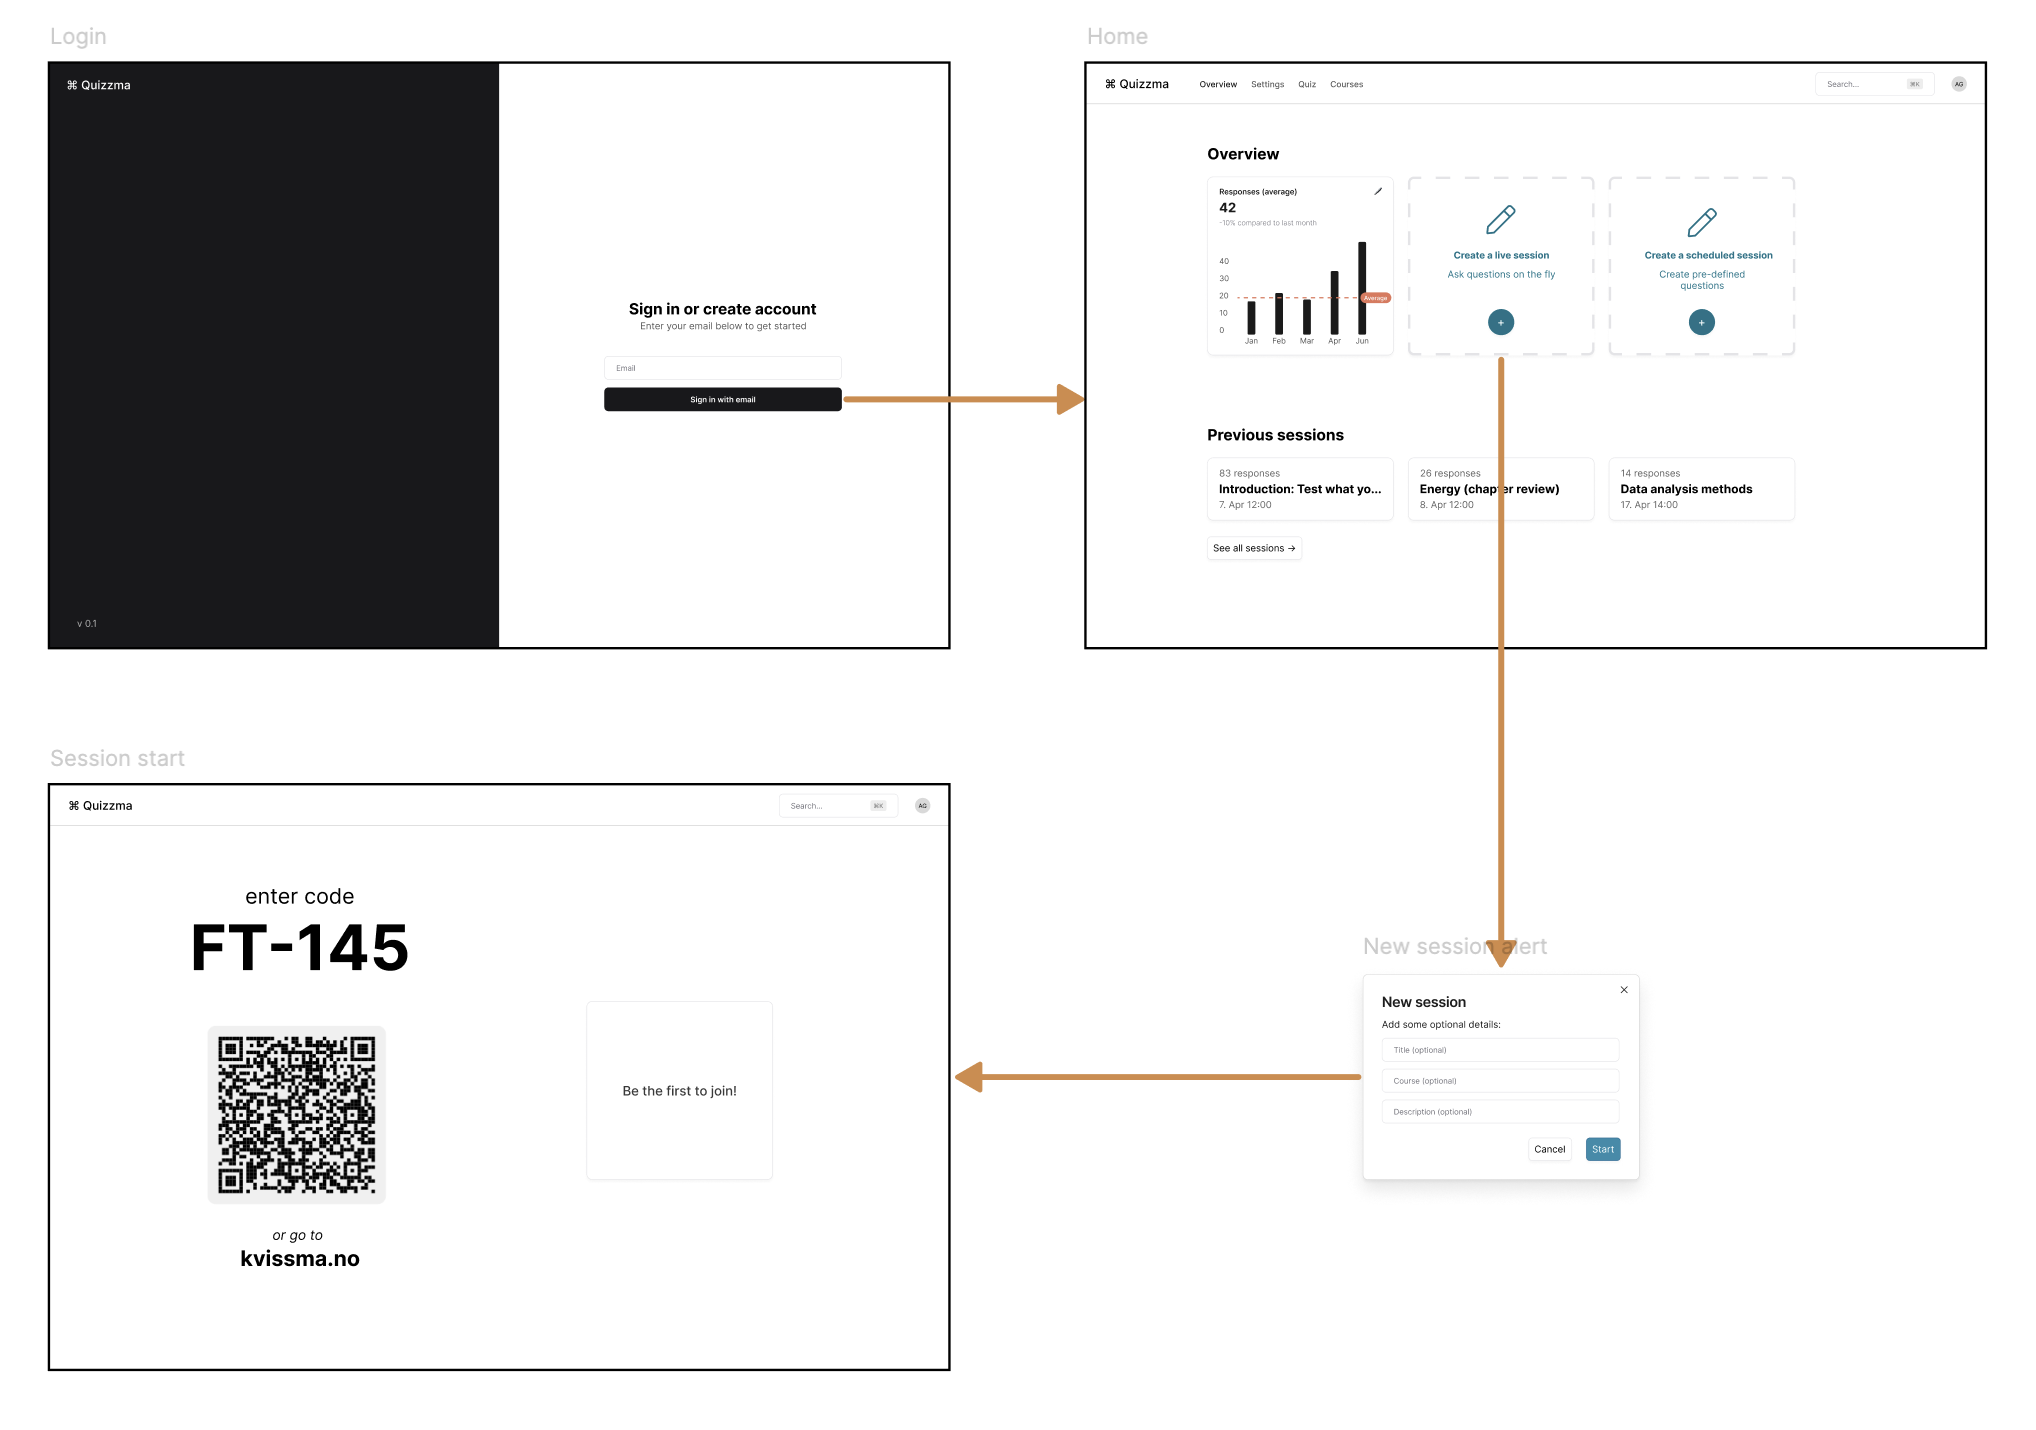
\includegraphics[width=1\linewidth]{figures//c5/host-frontend.png}
    \caption{Host frontend flow}
    \label{fig:host-frontend-flow}
\end{figure}

\begin{figure}[h!]
    \centering
    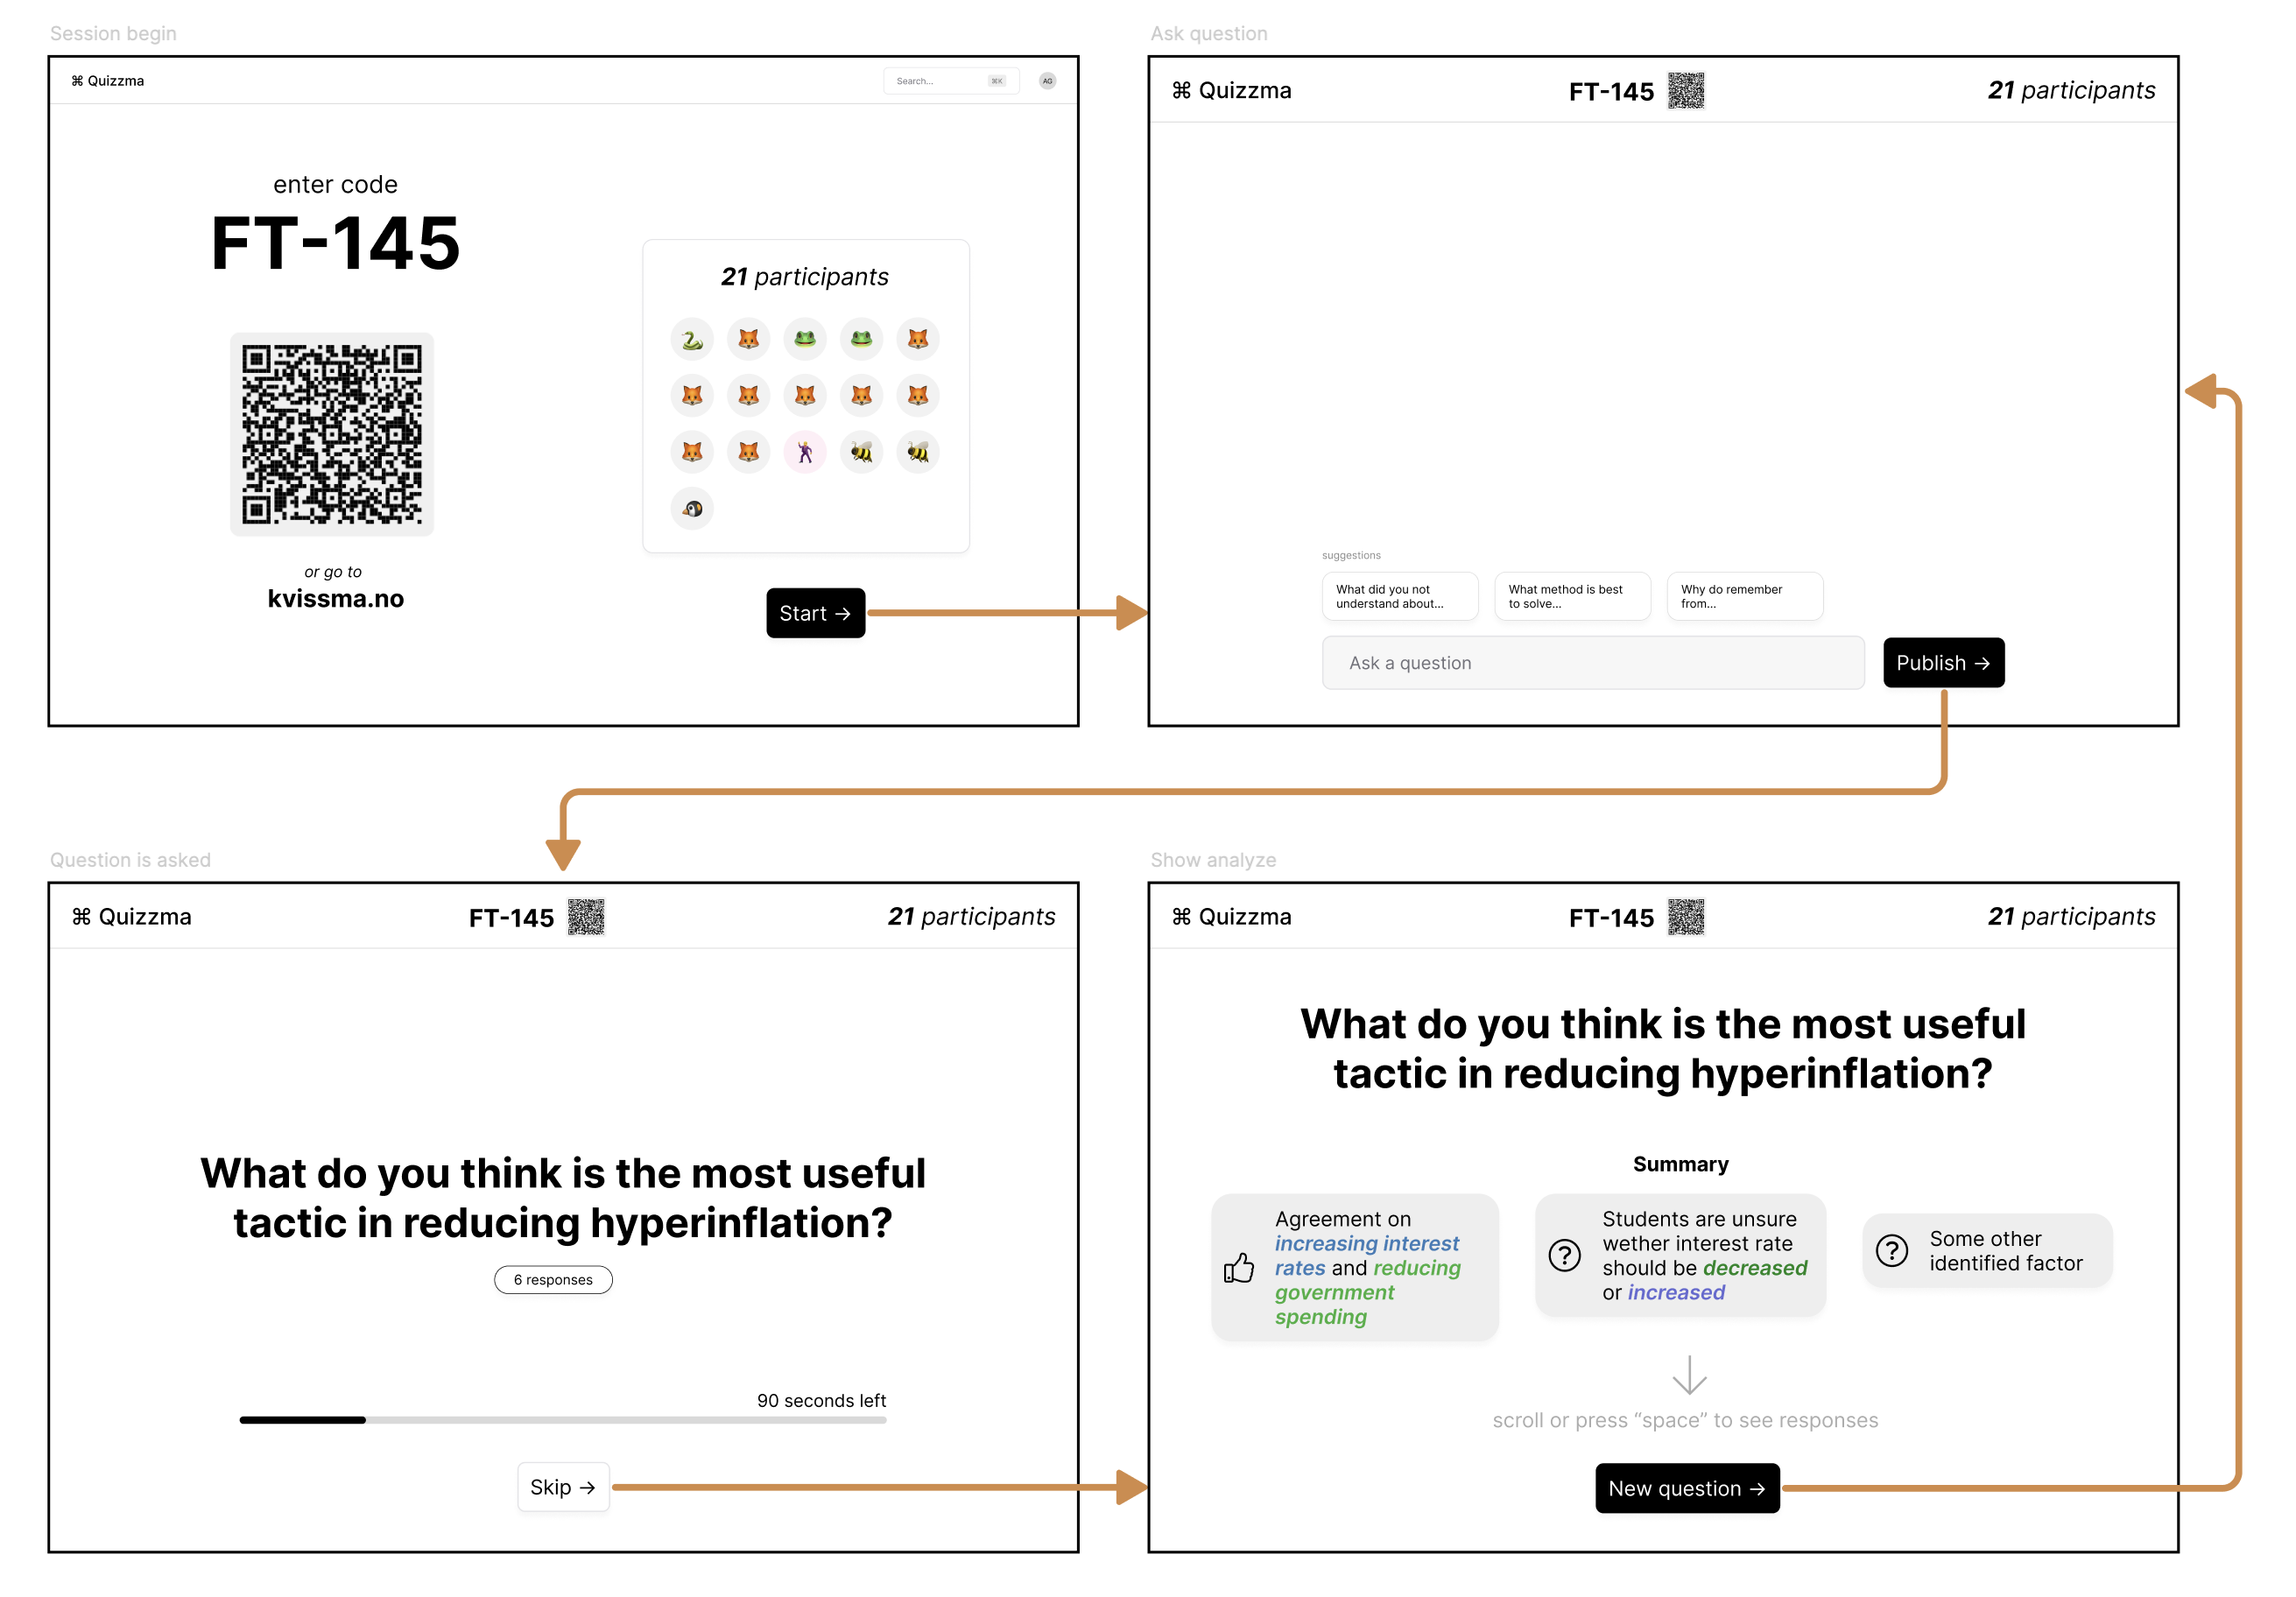
\includegraphics[width=1\linewidth]{figures//c5/session-frontend.png}
    \caption{A flowchart of how a session-host will function}
    \label{fig:session-host-flowchart}
\end{figure}

\subsection{Participant frontend}
This frontend will allow users to join sessions, answer questions, and provide a review of the service. Since the users will primarily use a smartphone, the development will prioritise ``mobile-first'' design. The frontend will allow users to join a session by submitting a session code (6 letters). The people who join the session will be able to answer questions anonymously. The frontend will have three main states after a user joins, namely 

\begin{enumerate}
    \item Waiting for a question
    \item Write a question
    \item Submit feedback
\end{enumerate}


\begin{figure}[h!]
    \centering
    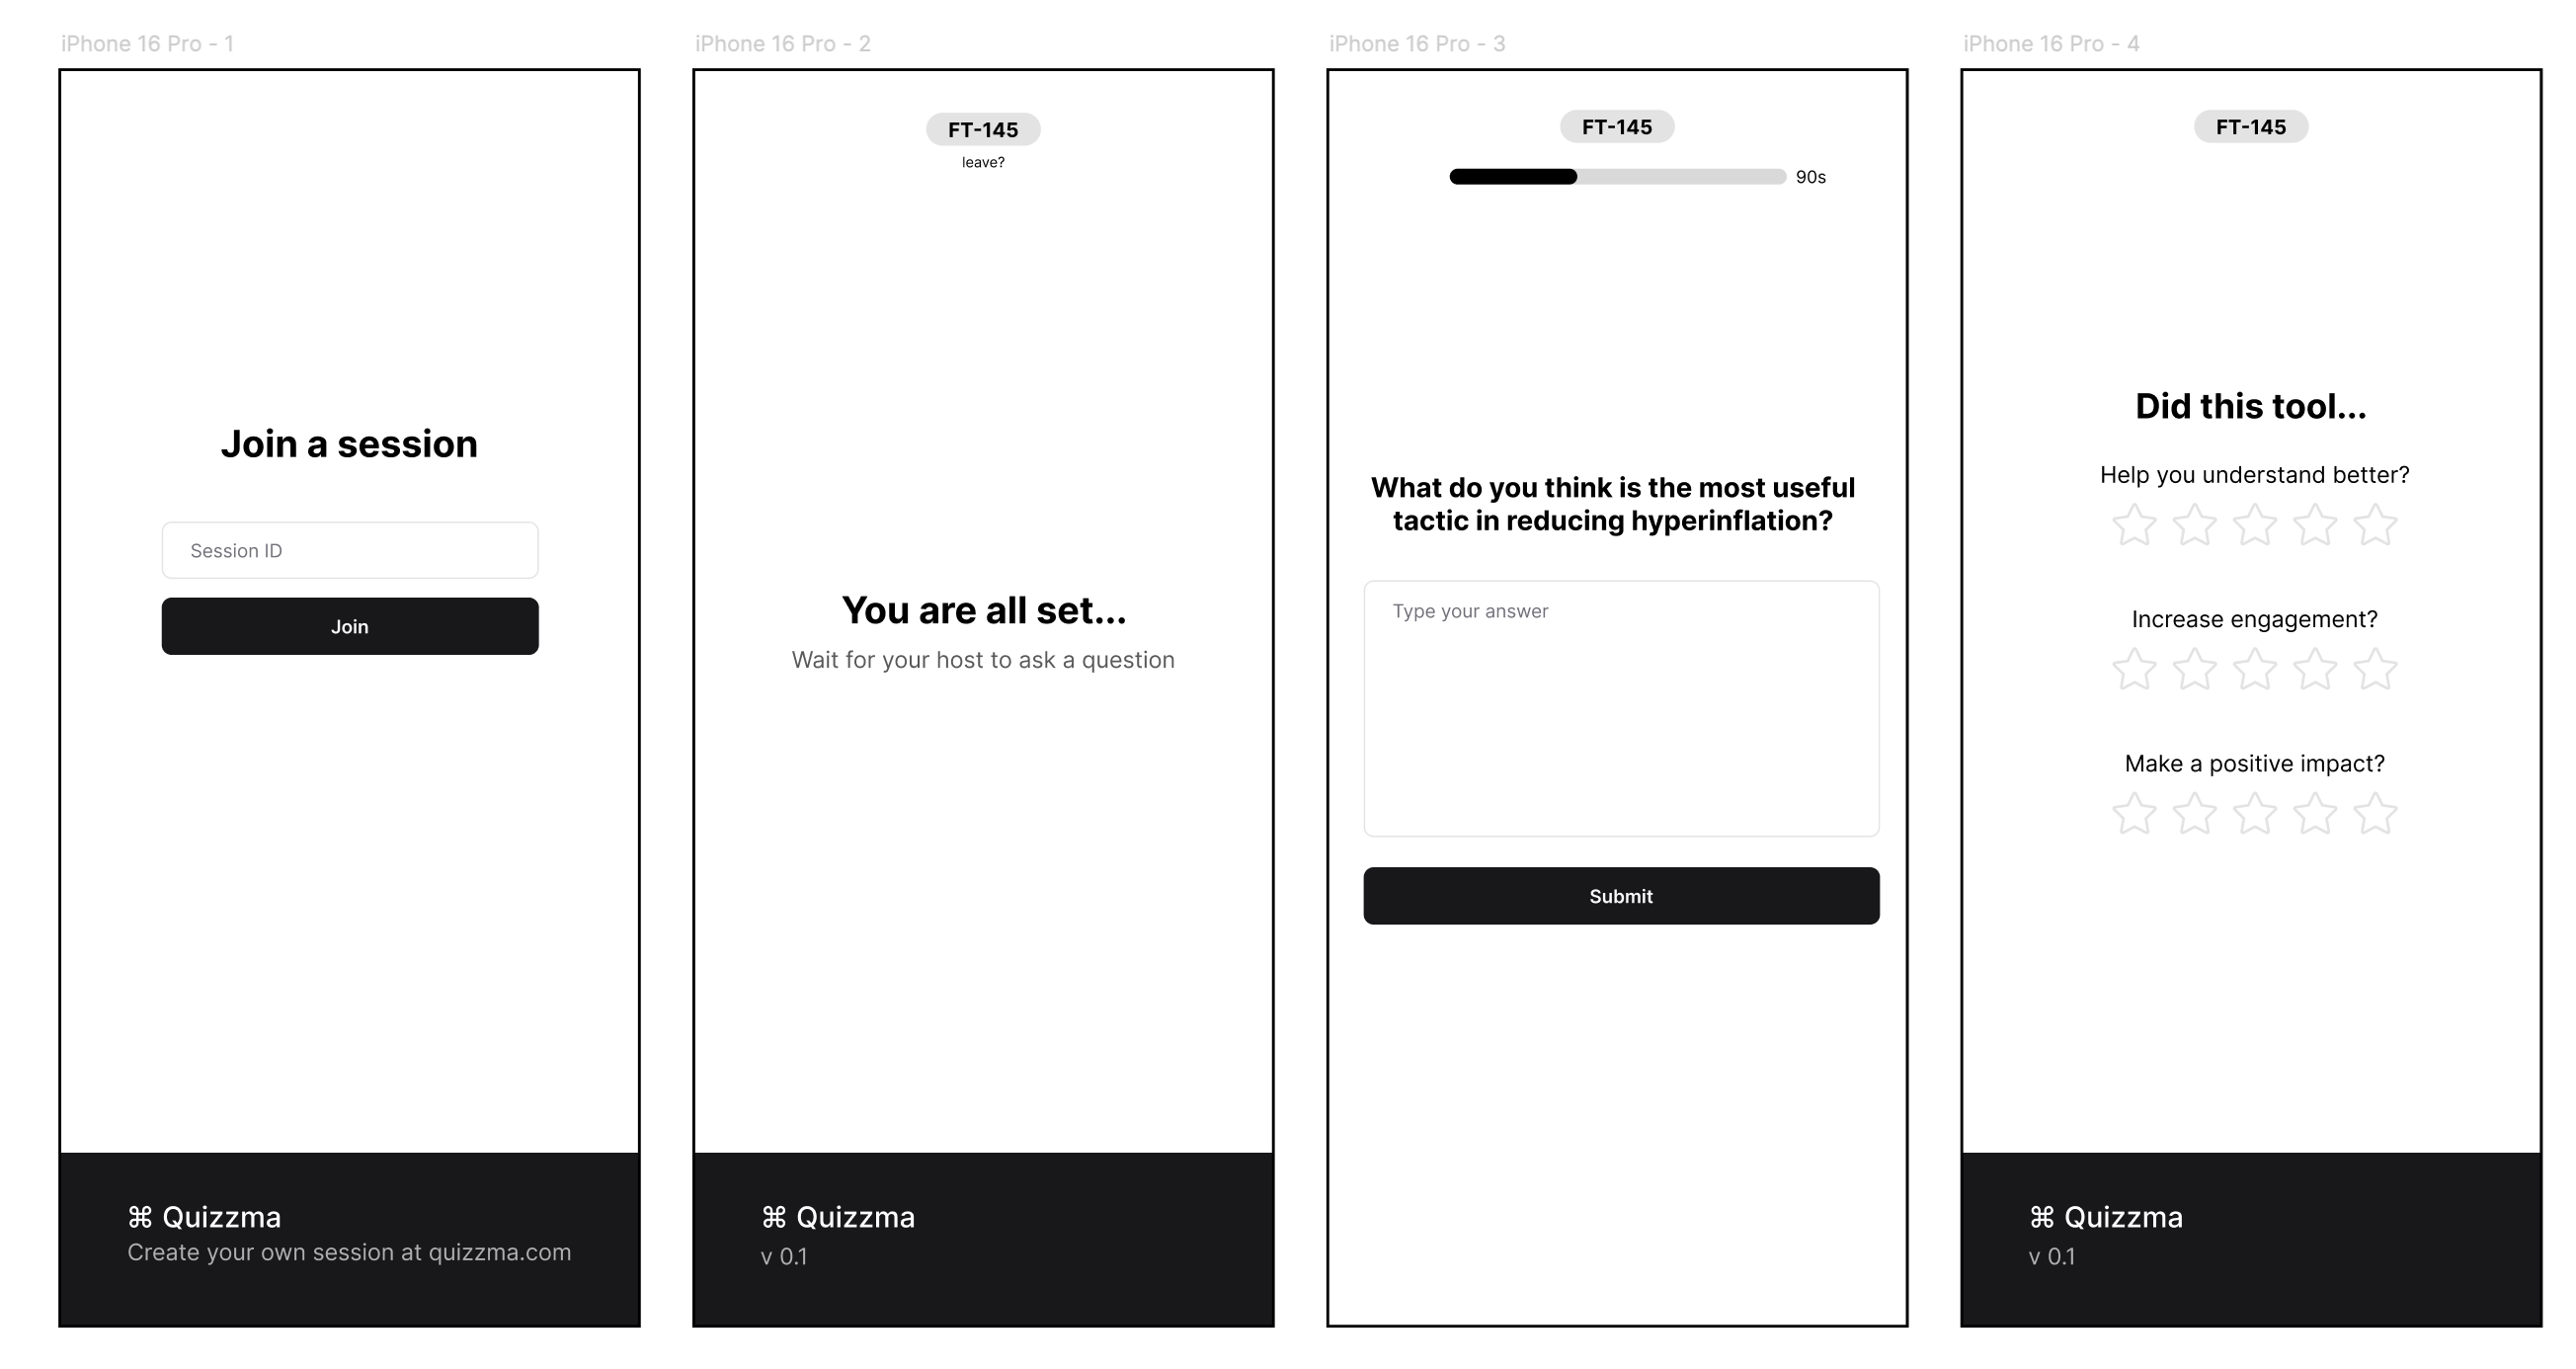
\includegraphics[width=1\linewidth]{figures//c5/user-frontend.png}
    \caption{Participant frontend screens}
    \label{fig:participant-frontend}
\end{figure}


\subsection{Backend}
We will also need to create a backend that can interact with our two frontends. It must handle the sessions and take care of processing the inputs. The backend will be written in Python, and we propose to use FastAPI with websockets to be able to stream answers to the session-host. We plan to use REST-ful practices for the users who submit answers, and let the backend handle the websockets so that analysis and results are updated in real-time. To simplify our approach, we will not use a database to store responses, but rather an in-memory storage solution.

We propose this simple approach to be able to make this prototype in enough time for the semester-start so that we can test in real classrooms as soon as possible. We find that more useful than having a performant and scalable solution. 

\begin{figure}[h!]
    \centering
    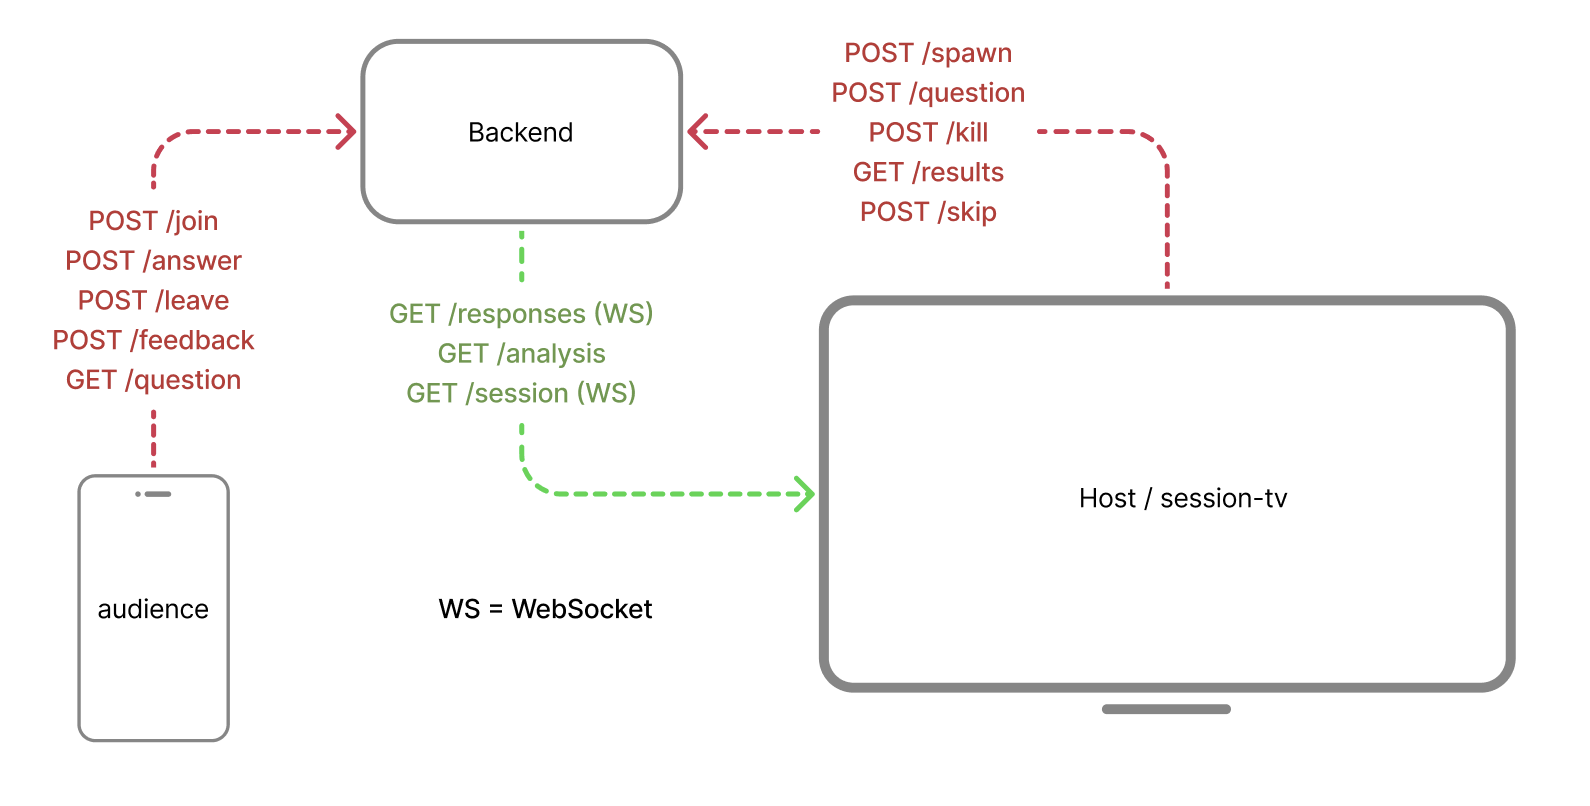
\includegraphics[width=1\linewidth]{figures//c5/backend.png}
    \caption{Possible backend endpoints}
    \label{fig:backend-endpoint-illustration}
\end{figure}

\subsection{Infrastructure}
We plan to host our backend on an NTNU hosted Linux virtual machine exposed internally to the NTNU network. This reduces the overhead of the session hosts, as they do not have to run the code locally for themselves. It will also be beneficial for privacy, as only NTNU-users will be allowed to access the website, reducing the potential for attacks and data leaks or exposure. In order to ensure enough performance - while not a primary concern - we believe it should be able to handle at least 200 responses a second. We plan to run API-tests (load tests) before deploying and testing this prototype. The reason is that we will limit our testing scope to classes on campus, and no classroom session will have enough students to send more responses than that.


\section{Testing of prototype}
To evaluate and test the performance of our prototype, we will conduct both a quantitative and qualitative analysis. While it is possible to measure the performance of our AI models and techniques directly by way of accuracy, precision or recall metrics, we believe that these are not sufficient to determine how our prototype performs as a Classroom Interaction Tool. Our evaluation will, therefore, not focus on the technical performance, but rather the practical utility and effectiveness of the tool itself. 

The actual testing of our prototype will happen live during real lectures. In addition to the core functionality of allowing student-teacher interaction, we plan to collect quantitative data in the form of student feedback after a session is complete. Then we gather qualitative data afterwards through interviews with both teachers and students.


\subsection{Qualitative analysis}
A professor or teacher will be provided with instructions from us on how to use our prototype in the classroom. Then the professor will use the system in a lecture. After the lecture is done we will determine the performance of our solution via in-depth interviews from teachers and students. We will try to identify the participants' perceived benefits and drawbacks of the system. We primarily want to identify if the system made lectures more engaging for students, simpler for the teacher and hopefully beneficial for the learning process and learning outcomes.

We plan to create an interview-guide that will be used to make structured interviews. We will focus on specific use cases, perceived benefits and challenges. These findings will hopefully identify whether the prototype is promising or if it requires more testing. We will also make sure to differentiate feedback between the solution as a concept, and feedback regarding the performance of our technical solutions. For instance while participants might enjoy the concept, our AI and other algorithms might require improvements in order to be felt as useful for the participants. In that case, the prototype itself might still be perceived as positive.


\subsection{Quantitative analysis}
For the quantitative analysis, we plan to implement a small questionnaire that will be shown to the students at the end of a session. The questions will be in the form of a likert-scale (1-5) and represented as stars. The screen can be seen in figure \ref{fig:participant-frontend}. We chose this feedback form to ensure it is as easy as possible for students to answer, and to avoid people not answering. This way we hope to get a lot of answers, at the cost of having few questions and no free-text input. 

The questions we ask:
\begin{enumerate}
    \item Did this tool help you understand better?
    \item Did this tool increase engagement?
    \item Did this tool make a positive impact?
\end{enumerate}

These questions are made to assess whether the tool enhanced the learning environment, increased engagement and/or improved comprehension. By combining the insights from both qualitative and quantitate data, we believe that we can get an understanding of the prototype's performance and potential for further development.

% Keep preliminary RQ as a goal instead of finding a concrete RQ

% \section{Preliminary research question for master thesis}
% \todo{Create a research question for next semester based on the findings}

% Suggestion: How to get actionable insights from students' open-text responses through the use of AI?